% L12a lecture companion. Notebook hashes and coverage are recorded in README.md.
% Style files and Cornell seal are copied unchanged from the L11c deck (identical
% to L10c, L10a, L9c, and L9a, which match the approved L6a deck). The two figures
% are the lecture's SVGs in ../figs, converted to light PDFs by `make figures`.
%
% Notation follows the lecture: the MDP tuple (S, A, R(s,a), T(s'|s,a), gamma),
% value functions U_k and U^*, the action values Q(s,a) and Q^*(s,a), the observed
% reward r and next state s', the learning rate alpha (alpha_n for the n-th update
% of a pair), the exploration probability epsilon, the policy pi, the number of
% episodes N, the step limit d, and the step counter t.
\documentclass[aspectratio=169,11pt]{beamer}
\usepackage{vnslides}
\renewcommand{\vnlecturecode}{L12a}
\newcommand{\lecturelink}{https://github.com/varnerlab/CHEME-5800-CourseRepository-Fall-2026/blob/main/weeks/week-12/L12a/CHEME-5800-L12a-Lecture-QLearning-Fall-2026.ipynb}
\newcommand{\examplelink}{https://github.com/varnerlab/CHEME-5800-CourseRepository-Fall-2026/blob/main/weeks/week-12/L12a/CHEME-5800-L12a-Example-QLearningGridWorld-Fall-2026.ipynb}
\newcommand{\lablink}{https://github.com/varnerlab/CHEME-5800-CourseRepository-Fall-2026/blob/main/weeks/week-12/L12b/CHEME-5800-L12b-Lab-AdaptiveDosing-QLearning-Fall-2026.ipynb}
\newcommand{\lecturesource}[1]{\note{[Sources]\par
  \href{\lecturelink}{L12a lecture: Model-Free Reinforcement Learning and Q-Learning.}\par
  #1\par[/Sources]}}
\newcommand{\Sset}{\mathcal S}
\newcommand{\Aset}{\mathcal A}

\title{\texorpdfstring{{\vnheavy L12a}: Model-Free Reinforcement Learning}{L12a: Model-Free Reinforcement Learning}}
\subtitle{\texorpdfstring{Q-learning\\[3pt]CHEME 5800 Cornell University}{Q-learning; CHEME 5800 Cornell University}}
\author{Copyright Jeffrey Varner 2026. All Rights Reserved}

\begin{document}
\special{pdf:minorversion 7}
\vntitlepage

\begin{frame}{Objectives for Today}
  How can an agent learn to act well when it has no model of its environment?

  \vspace{0.4em}
  {\large\textbf{\ink{Today's concepts}}}
  \vspace{0.2em}
  \begin{itemize}\setlength{\itemsep}{0.4em}
    \item \hilite{Describe the reinforcement learning problem}: an agent takes
      an action, then sees a reward and a new state, without knowing the rules.
    \item \hilite{Update action values from experience}: after each
      step, Q-learning corrects one action value toward what the agent observed.
    \item \hilite{Explain when Q-learning converges}: Q-learning needs every
      action tried again and again, and a learning rate that shrinks at the
      right pace.
  \end{itemize}
  \slidenote{Lecture:}{\href{\lecturelink}{Model-Free Reinforcement Learning and Q-Learning}}
  \lecturesource{Introduction and three Learning Objectives.}
\end{frame}

\begin{frame}{Lecture and Example}
  \textbf{\ink{Lecture:}}
  \href{\lecturelink}{Model-Free Reinforcement Learning and Q-Learning}

  In this lecture, we write the Q-learning update rule, assemble it into the
  Q-learning algorithm, and state when Q-learning converges.

  \vspace{1.1em}
  \textbf{\ink{Example:}}
  \href{\examplelink}{Q-Learning in the Lava Grid World}

  In this example, a roomba that has finished cleaning the kitchen learns to
  return to its charging station without falling into a lava pit. We train the
  roomba with Q-learning, then compare its policy with the optimal policy from
  value iteration.
  \lecturesource{Examples section.}
\end{frame}

\begin{frame}{The Reinforcement Learning Problem}
  How does an agent learn the best action in each state when it does not know
  the rules of its world?

  \vspace{0.2em}
  \centering
  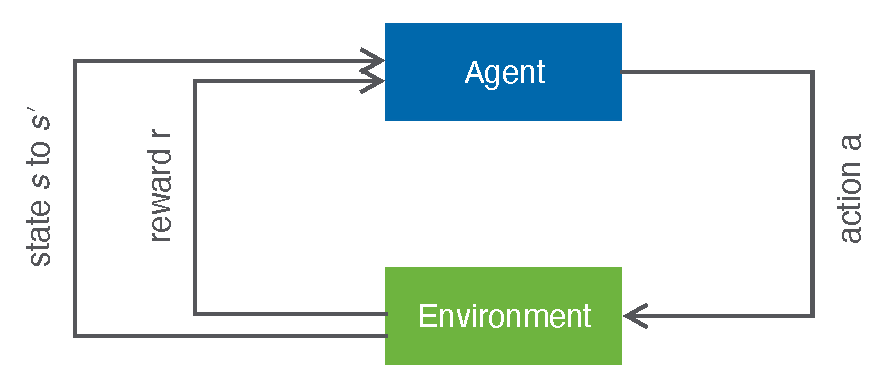
\includegraphics[width=\textwidth,height=0.52\paperheight,keepaspectratio]{assets/Fig-Schematic-RL.pdf}

  \vspace{0.2em}
  \raggedright
  The agent observes its current state $s$ and selects an action $a$. The
  environment answers with a reward $r$ and the next state $s'$.
  \lecturesource{Reinforcement Learning Problem: opening paragraph and the agent-environment figure.
    Figure: ../figs/Fig-Schematic-RL.svg, converted to a light PDF.}
\end{frame}

\begin{frame}{Learning from Interaction}
  We have seen two approaches to learning from interaction:

  \vspace{0.3em}
  \begin{itemize}\setlength{\itemsep}{0.5em}
    \item \hilite{Multiplicative weights} adjusts the probability of each
      action from its past performance. It does nearly as well as the best
      fixed action in hindsight.
    \item \hilite{Bandit algorithms} work without states. In each round, they
      estimate the reward of each action and adapt how they choose.
    \item \hilite{Q-learning} adds the state. It estimates the long-term value
      of each state-action pair, which lets the agent learn when its actions
      change what happens next.
  \end{itemize}

  \vspace{0.5em}
  All three balance exploring new actions to gather information against
  exploiting known actions to collect reward.
  \lecturesource{Reinforcement Learning Problem: the two earlier approaches and the Q-learning paragraph.}
\end{frame}

\begin{frame}{From Value Iteration to Action Values}
  A Markov decision process (MDP) is the tuple
  $\left(\Sset,\Aset,R(s,a),T(s'\,|\,s,a),\gamma\right)$ of states, actions,
  rewards, transition probabilities, and a discount factor. Value iteration
  computes the optimal value function $U^{*}(s)$ by repeating the
  \hilite{Bellman backup} in sweeps $k$:
  \[
    U_{k+1}(s)=\max_{a\in\Aset}\Bigl(\underbrace{R(s,a)}_{\text{now}}+
    \gamma\overbrace{\sum_{s'\in\Sset}T(s'\,|\,s,a)\,U_k(s')}^{\text{future}}\Bigr)
  \]

  We write the \hilite{action-value function}, also called the Q-function, in
  terms of $U^{*}$:
  \[
    Q^{*}(s,a)=R(s,a)+\gamma\sum_{s'\in\Sset}T(s'\,|\,s,a)\,\underbrace{U^{*}(s')}_{=\,\max_{a'\in\Aset}Q^{*}(s',a')}
  \]

  $Q^{*}(s,a)$ is the value of taking action $a$ in state $s$: the reward now
  plus the discounted expected value of the next state.
  \lecturesource{From Value Iteration to Action Values: the Bellman backup and the action-value function.}
\end{frame}

\begin{frame}{The Q-Table}
  We store the action values in a table, the \hilite{Q-table}, with one row per
  state and one column per action.

  \vspace{0.2em}
  \centering
  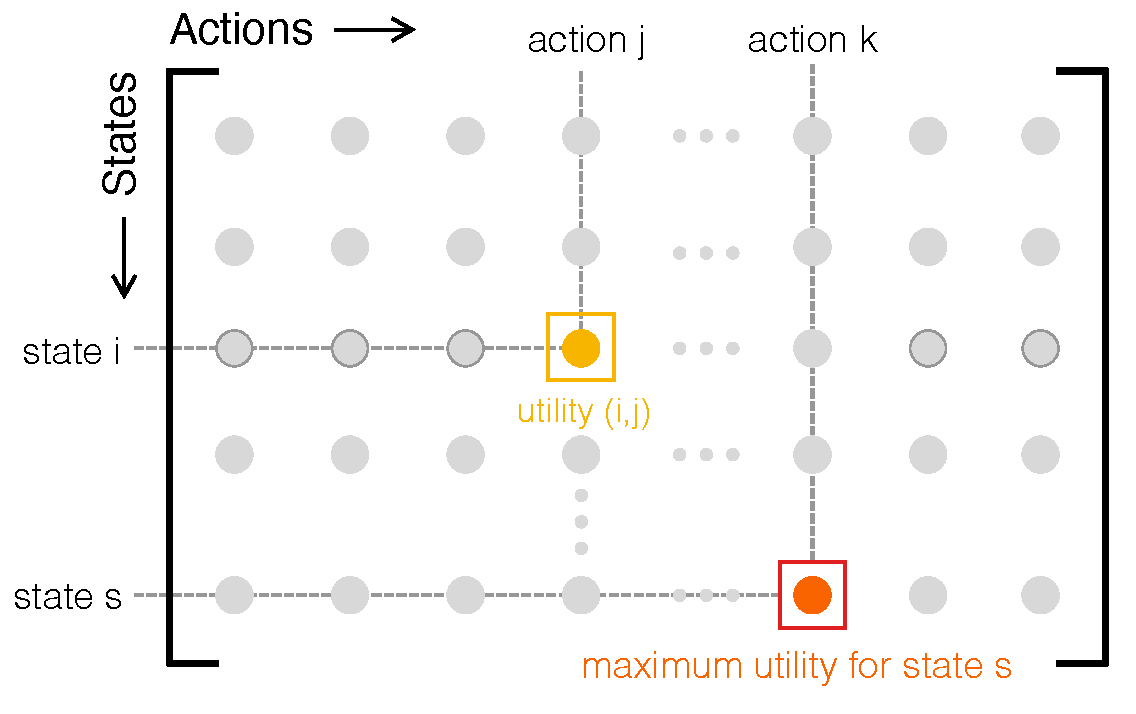
\includegraphics[width=\textwidth,height=0.46\paperheight,keepaspectratio]{assets/Fig-Q-Schematic.pdf}

  \vspace{0.2em}
  \raggedright
  The policy reads each row and picks the column with the largest entry.
  \lecturesource{The Q-table caption.
    Figure: ../figs/Fig-Q-Schematic.svg, converted to a light PDF.}
\end{frame}

\begin{frame}{What Value Iteration Needs}
  Value iteration uses the reward function $R(s,a)$ and the transition model
  $T(s'\,|\,s,a)$:

  \vspace{0.3em}
  \begin{itemize}\setlength{\itemsep}{0.5em}
    \item With $R$ and $T$, value iteration requires
      $\mathcal O(|\Sset|^{2}\,|\Aset|)$ operations per sweep.
    \item Without $R$ and $T$, the usual case for a real robot, a reactor, or a
      patient, what can we do?
  \end{itemize}

  \vspace{0.5em}
  Let's think of the Q-table as the agent's \hilite{memory}. The agent can then
  learn to act optimally by updating its memory after each step from the
  outcomes of its actions, without $T$ or $R$.
  \lecturesource{From Value Iteration to Action Values: the paragraph on what value iteration uses and the memory paragraph.}
\end{frame}

\begin{frame}{The Q-Learning Update}
  Q-learning (\href{https://www.cs.rhul.ac.uk/~chrisw/new_thesis.pdf}{Watkins,
  1989}) estimates $Q(s,a)$ from repeated experiments. In each experiment, the
  agent in state $s$ takes action $a$, receives a reward $r$, and moves to a
  state $s'$.

  \vspace{0.3em}
  After each experiment, the agent updates one entry of the Q-table:
  \[
    Q(s,a)\gets\underbrace{Q(s,a)}_{\text{old value}}+\alpha\cdot
    \underbrace{\left(\overbrace{r+\gamma\cdot\max_{a'\in\Aset}Q(s',a')}^{\text{target}}-Q(s,a)\right)}_{\text{net new information}}
  \]

  where $0<\alpha\le1$ is the learning rate and $0\le\gamma<1$ is the discount
  factor. Every other entry keeps its value.
  \lecturesource{Q-Learning: opening paragraphs and the update rule.}
\end{frame}

\begin{frame}{The Update as a Weighted Average}
  The update is also a weighted average of the old value and the target:
  \[
    Q(s,a)\gets(1-\alpha)\cdot\underbrace{Q(s,a)}_{\text{old value}}+\alpha\cdot
    \underbrace{\left(r+\gamma\cdot\max_{a'\in\Aset}Q(s',a')\right)}_{\text{target}}
  \]

  \vspace{0.5em}
  We estimate the policy $\pi:\Sset\to\Aset$ by selecting the action that
  maximizes $Q(s,a)$ in each state $s$:
  \[
    \pi(s)=\arg\max_{a\in\Aset}Q(s,a)
  \]
  \lecturesource{Q-Learning: the weighted-average form of the update and the policy.}
\end{frame}

\begin{frame}{Episodes and Epsilon-Greedy Actions}
  Q-learning runs in \hilite{episodes}. Each episode runs until the agent enters
  an absorbing state or reaches a step limit.

  \vspace{0.4em}
  Each step chooses an action with the \hilite{epsilon-greedy} rule:
  \begin{itemize}\setlength{\itemsep}{0.3em}
    \item With probability $\epsilon$, the agent explores with a random action.
    \item Otherwise, the agent exploits the action with the largest current
      value.
  \end{itemize}

  \vspace{0.4em}
  \emph{Related to bandits?} Each row of the Q-table acts like its own bandit,
  and epsilon-greedy is a bandit rule. Other bandit rules, such as UCB1, can
  replace it, as long as every action in every state keeps being tried.
  \lecturesource{Algorithm: episodes, the epsilon-greedy rule, and the note on bandits.}
\end{frame}

\begin{frame}{Q-Learning Algorithm}
  \small
  \textbf{Initialize}: Given $\Sset$, $\Aset$, the absorbing states,
  $0\le\gamma<1$, $0<\alpha\le1$, $0\le\epsilon\le1$, a number of episodes
  $N\ge1$, and a step limit $d\ge1$, set $Q(s,a)\gets0$ for all $s$ and $a$.

  \vspace{0.2em}
  For $i=1$ to $N$ \textbf{do}:
  \begin{enumerate}\setlength{\itemsep}{0.1em}
    \item Choose a starting state $s$ that is not absorbing, and set $t\gets0$.
    \item While $s$ is not absorbing and $t<d$ \textbf{do}:
      \begin{itemize}\setlength{\itemsep}{0.05em}
        \item Choose the action $a$: roll a random number $p\in[0,1]$.
          \begin{itemize}\setlength{\itemsep}{0em}
            \item If $p\le\epsilon$ \textbf{then} choose $a\in\Aset$ uniformly
              at random (exploration).
            \item Otherwise, choose $a\gets\arg\max_{a'\in\Aset}Q(s,a')$
              (exploitation).
          \end{itemize}
        \item Take action $a$, and observe $r$ and $s'$ from the world.
        \item Update
          $Q(s,a)\gets Q(s,a)+\alpha\left(r+\gamma\max_{a'\in\Aset}Q(s',a')-Q(s,a)\right)$.
        \item Update $s\gets s'$ and $t\gets t+1$.
      \end{itemize}
  \end{enumerate}

  \vspace{0.1em}
  \textbf{Extract Policy}: for each $s\in\Sset$, compute
  $\pi(s)\gets\arg\max_{a\in\Aset}Q(s,a)$.
  \lecturesource{Algorithm: the Initialize/For/While pseudocode and Extract Policy. The Given list is shortened to symbols defined on earlier slides.}
\end{frame}

\begin{frame}{Absorbing States}
  An episode ends as soon as the agent enters an absorbing state:

  \vspace{0.3em}
  \begin{itemize}\setlength{\itemsep}{0.5em}
    \item The agent never updates the rows of $Q$ that belong to absorbing
      states. Those rows stay at zero.
    \item The target of a move into an absorbing state is just its reward $r$,
      with no future to add.
  \end{itemize}
  \lecturesource{Algorithm: the closing paragraph on absorbing states.}
\end{frame}

\begin{frame}{When Does Q-Learning Converge?}
  Q-learning converges to the optimal action values, $Q(s,a)\to Q^{*}(s,a)$,
  with probability one
  (\href{https://doi.org/10.1007/BF00992698}{Watkins and Dayan, 1992}). The
  environment must have the Markov property, and three conditions must hold:

  \vspace{0.3em}
  \begin{itemize}\setlength{\itemsep}{0.45em}
    \item \hilite{Finite, fixed MDP and discounting}: the states and actions
      are finite, the rewards are bounded, the rewards and transition
      probabilities do not change, and $0\le\gamma<1$.
    \item \hilite{Learning rate decay}: the learning rate $\alpha_n(s,a)$ of
      the $n$-th update of each pair satisfies
      $\sum_{n=1}^{\infty}\alpha_n(s,a)=\infty$ and
      $\sum_{n=1}^{\infty}\alpha_n^{2}(s,a)<\infty$.
    \item \hilite{Infinite exploration}: every state-action pair of a state
      that is not absorbing is visited, and updated, infinitely often.
  \end{itemize}
  \lecturesource{Convergence: the three conditions.}
\end{frame}

\begin{frame}{Meeting the Conditions}
  \begin{itemize}\setlength{\itemsep}{0.6em}
    \item The first sum lets the updates carry $Q(s,a)$ as far from its
      starting value as it needs to go. The second sum makes the noise of the
      individual targets average out.
    \item The choice $\alpha_n(s,a)=1/n$ satisfies both sums. With this choice,
      $Q(s,a)$ is the running average of the targets the pair has seen.
    \item Epsilon-greedy selection with a fixed $\epsilon>0$, together with
      episodes that start at random in any state that is not absorbing, meets
      the exploration condition.
  \end{itemize}

  \vspace{0.5em}
  The greedy policy is already correct once the best action in each state has
  the largest estimate.
  \lecturesource{Convergence: the paragraphs under the learning rate decay and infinite exploration bullets, and the closing sentence on the greedy policy.}
\end{frame}

\begin{frame}{Caveats and Practical Notes}
  Of the convergence conditions, infinite exploration is the hardest to meet in
  practice:

  \vspace{0.3em}
  \begin{itemize}\setlength{\itemsep}{0.45em}
    \item \hilite{Exploration schedule}: if $\epsilon$ is too small, or shrinks
      too quickly, the agent can settle on a poor action. If $\epsilon$ stays
      large, the agent wastes many steps on random actions.
    \item \hilite{Sparse and delayed rewards}: when few pairs earn a nonzero
      reward, a new agent may take many steps before its first reward. Later
      visits can carry that reward back one step at a time. Reward shaping adds
      small rewards that guide the agent toward the goal.
    \item \hilite{Rate of convergence}: every state-action pair needs many
      visits, and the number of experiments grows with the size of the table.
      When $R$ and $T$ are known, value iteration is usually faster.
  \end{itemize}
  \lecturesource{Caveats \& Practical Notes: the three issues.}
\end{frame}

\begin{frame}{Example: Q-Learning in the Lava Grid World}
  In this example, a roomba that has finished cleaning the kitchen must return
  to its charging station without falling into a lava pit:

  \vspace{0.5em}
  \begin{enumerate}\setlength{\itemsep}{0.5em}
    \item Build the lava grid world, and a function that returns the next square
      and the reward of one move.
    \item Train the roomba with Q-learning.
    \item Compare the learned policy with the optimal policy from value
      iteration, and follow both from a starting square.
  \end{enumerate}

  \vspace{0.5em}
  After 2000 episodes, both policies reach the station from $(20,20)$ in 33
  moves, by different routes.
  \slidenote{Example:}{\href{\examplelink}{Q-learning in the lava grid world}}
  \lecturesource{Caveats \& Practical Notes: the example box. Companion example: Tasks 1--3 and the second key takeaway.}
\end{frame}

\begin{frame}{Lab: Adaptive Drug Dosing with Q-Learning}
  In the \href{\lablink}{lab}, we treat a course of chemotherapy as a Markov
  decision process in which we choose a drug dose each treatment cycle:

  \vspace{0.5em}
  \begin{itemize}\setlength{\itemsep}{0.5em}
    \item The state is the size of the tumor and the level of toxicity, the
      damage the drug does to healthy tissue. Each action is a drug dose.
    \item Value iteration computes the optimal dosing policy, which serves as
      the benchmark.
    \item You will write the Q-learning update, train an agent on simulated
      treatment cycles, and compare its doses with the optimal ones.
  \end{itemize}
  \slidenote{Lab:}{\href{\lablink}{Adaptive drug dosing with Q-learning}}
  \lecturesource{Lab section. Lab notebook: introduction and Learning Objectives.}
\end{frame}

\begin{frame}{Summary}
  We developed model-free reinforcement learning, in which an agent learns how
  to act from the rewards it receives.

  \vspace{0.5em}
  {\large\textbf{\ink{Key takeaways}}}
  \vspace{0.3em}
  \begin{itemize}\setlength{\itemsep}{0.6em}
    \item \textbf{\ink{Model-free learning.}} The agent learns from the states,
      actions, and rewards it observes, without a model.
    \item \textbf{\ink{Q-learning.}} Each step moves one action value toward a
      target built from the observed reward and next state.
    \item \textbf{\ink{Convergence.}} Every pair needs visits again and again,
      and a learning rate that shrinks at the right pace.
  \end{itemize}

  \vspace{0.5em}
  Reinforcement learning lets an agent learn good behavior through trial and
  error, even when no one can write down the rules of its environment.
  \lecturesource{Summary: three key takeaways and the closing sentence.}
\end{frame}

\end{document}
